%-----------------------------------------------------------------------------
%
%               Template for sigplanconf LaTeX Class
%
% Name:         sigplanconf-template.tex
%
% Purpose:      A template for sigplanconf.cls, which is a LaTeX 2e class
%               file for SIGPLAN conference proceedings.
%
% Guide:        Refer to "Author's Guide to the ACM SIGPLAN Class,"
%               sigplanconf-guide.pdf
%
% Author:       Paul C. Anagnostopoulos
%               Windfall Software
%               978 371-2316
%               paul@windfall.com
%
% Created:      15 February 2005
%
%-----------------------------------------------------------------------------


%\documentclass[preprint]{sigplanconf}
\documentclass[11pt]{sigplanconf}

% The following \documentclass options may be useful:
%
% 10pt          To set in 10-point type instead of 9-point.
% 11pt          To set in 11-point type instead of 9-point.
% authoryear    To obtain author/year citation style instead of numeric.

\usepackage{yfonts}
\usepackage{amsmath}
\usepackage{amsthm}
\usepackage{amssymb}
%\usepackage{mathpartir}
\usepackage[colorlinks=true,
citecolor=citec,
linkcolor=linkc,
urlcolor=urlc,
]{hyperref}
\usepackage{url}
\usepackage{graphics}
\usepackage{graphicx}
\usepackage{wasysym}
\usepackage{harmony}
\usepackage{marvosym}
\usepackage{multirow}
\usepackage{xspace}
\usepackage[nameinlink,nosort]{cleveref}
\usepackage{xeCJK}
\usepackage[usenames,dvipsnames]{xcolor}
\usepackage[utopia]{mathdesign}
\usepackage{natbib}
\usepackage{ulem}
\usepackage[mathcal]{euscript}
\usepackage[linesnumbered,ruled]{algorithm2e}

\renewcommand{\UrlBreaks}{\do\/\do\a\do\b\do\c\do\d\do\e\do\f\do\g\do\h\do\i\do\j\do\k\do\l\do\m\do\n\do\o\do\p\do\q\do\r\do\s\do\t\do\u\do\v\do\w\do\x\do\y\do\z}


% ____________________________________________________________
% Listings Package Configuration
% \usepackage[scaled]{beramono}

%\renewcommand*\ttdefault{txtt}
\usepackage[T1]{fontenc}
% \usepackage{inconsolata}

\definecolor{citec}{RGB}{128,0,64}
\definecolor{linkc}{RGB}{0,64,128}
\definecolor{urlc} {RGB}{128,64,0}

\setCJKmainfont{HeiseiMinStd-W5}[Path = ./]
\setmonofont{Inconsolata-Regular}[Path = ./]

\newfontfamily\birbaslo{BirbasloText}[Path = ./]

% This Deep Tex Voodoo is from
%   <http://www.latex-community.org/forum/viewtopic.php?f=5&t=2072>
% It's purpose is to make \lstinline normal size, without affecting
% \lstinputlisting.  It seems to work but I have no idea how or why,
% and I rather hope never to learn.
%\makeatletter
%\lst@AddToHook{TextStyle}{\let\lst@basicstyle\ttfamily\normalsize}
%\makeatother

\begin{document}

\conferenceinfo{{\birbaslo sigbovik~'20}}{pittsburgh, PA, USA}
\copyrightyear{2020}
\copyrightdata{}

\title{
% how to \texttt{git bisect} when your test suite hates you
% how to \texttt{git bisect} when your test suite is a hater
how to \texttt{git bisect} when your test suite is having a bad day
% how to {\tt git bisect} when yr test suite is just, trying its best ok % there we go
}
% \subtitle{\em The Randomly-Scoped Lambda Calculus}
% \subtitle{Subtitle Text, if any}
% \subtitle{a probability puzzle}

\authorinfo{ben blum}{}{bblum@alumni.cmu.edu}

\maketitle

\begin{abstract}
	I like probability puzzles but don't know enough stats to actually solve them properly
	so I threw some thinking sand at it and learned some interesting stuff anyway.
\end{abstract}

% \category{D.D.R.}{Exercise and Fitness}{Arcade Dance Games}

\keywords pdflatex
% bracket, groove, in, jumps, the

\newcommand\confidents{\ensuremath{\mathcal{Z}}\xspace}
\newcommand\pdf{\ensuremath{\mathsf{pdf}}\xspace}
\newcommand\cdf{\ensuremath{\mathsf{cdf}}\xspace}

\section{problem statement}

Let's say you're trying to bisect
% a bug in
a given range of $n$ commits.%
\footnote{To use binary search to find a commit that introduced a bug.}
Call them $c_0 \dots c_{n-1}$, where $c_0$ is known safe and $c_n$ is known to have the bug.
You'd probably start by testing $c_{n/2}$, right?
And you'd expect to pinpoint the buggy comit in $\log_2(n)$ steps.
That's math.

Ok, but what if the bug reprodues nondeterministically with some probability $p<1$.
You can't even pinpoint the bug at some $c_{b}$ for sure anymore;
you can at best know
that it \textasciitilde{}prooobably\textasciitilde~won't reproduce in any $c_{i<b}$,
with some confidence $\confidents$.
Now evaluate your strategy by the expected number of steps to achieve, let's say for tradition's sake, $\confidents \ge 0.99999$.
Is it still optimal to bisect at the midpoint?%
\footnote{Spoiler: No, or I wouldn't have bothered with this paper.}
What would be a better strategy, as a function of $p$?

%%%%%%%%%%%%%%%%%%%%%%%%%%%%%%%%%%%%%%%%%%%%%%%%%%%%%%%%%%%%%%%%%%%%%%%%%%%%%%%%

\section{intermission}

Put the paper on pause now and think about it.
No, really, give it a go!
I mean, if you don't think math puzzles like this are cool, just stop reading, no worries.
I'm sure there's a paper about, like, hygienic image macros or empire machines or something for you just a few page-turns away.
% I'm sure tom7 is up to some wacky hijinks or something just a few page-turns away.

If you're feeling adventurous,
implement a strategy and throw it in this simulator I implemented to see how it stacks up:
\url{https://github.com/bblum/sigbovik/blob/master/bisect}.
You just gotta implement {\tt trait BisectStrategy},
and it even does all the hard work of applying Bayes's rule
%computing the
%distribution of
%priors with Bayes's rule
for you and letting you see the PDF and everything.
Check it out.


%%%%%%%%%%%%%%%%%%%%%%%%%%%%%%%%%%%%%%%%%%%%%%%%%%%%%%%%%%%%%%%%%%%%%%%%%%%%%%%%

\section{pdfs, but not the portable document format kind, and our friend rev. bayes}

Ok, so let's model the problem as a sequence of steps on a probability distribution function
(henceforth, PDF; and also, CDF for the cumulative kind).
Initially, $\pdf(i) = 1/n$ for all $0 \le i < n$.
When the bug reproduces at some commit $b$,
you're certain no $c_{i>b}$ introduced the bug, so $\pdf(i>b) = 0$,
and $\pdf(i\le b)$ renormalizes as $1/b$, to satisfy the $\int \pdf(i) \text{d} i = 1$ invariant.%
\footnote{Implemented as {\tt fn adjust\_pdf\_bug\_repros()} in the simulator.}

In the deterministic case ($p=1$),
the symmetric thing happens when the test passes at some $c_j$: $\pdf(i\le j) = 0$.
But when $p<1$, we must generalized it \cite{mario3}. Bayes's rule provides that:
\[
P(A|B) = \frac{P(B|A) \times P(A)}{P(B)}
\]

\newcommand\renorm[1]{\ensuremath{\mathcal{R}_{#1}}\xspace}

In this case, $B$ is that the test passed at $c_j$, and $A$ is that bug be present at or before $c_j$ after all.
$P(B|A)$ is simply $1-p$.
$P(A)$ is the prior on $c_j$ containing the bug, i.e., $\cdf(j)$.
And $P(B)$ is the false negative probability weighted by the bug existing, i.e., $(1-p)\cdf(j) + 1(1-\cdf(j))$.
% simplifies to: cdf(j) - p*cdf(j) + 1 - cdf(j)
% simplifies to: 1 - p*cdf(j)
To update our priors on commits up to $j$, we renormalize by dividing out the old $\cdf(j)$
and multiplying by the new $P(A|B)$, i.e.,
%To update our priors on commits up to $j$, we divide out the old $\cdf(j)$
%and multiply by the new $P(A|B)$.
%Call this renormalization factor $\renorm{j}{i}$.
%\[
%	\forall i \le j \Rightarrow \renorm{i}{i} = 
%	\frac{1}{\cdf(j)}
%	\frac{(1-p)\cdf(j)}{(1-p)\cdf(j) + (1-\cdf(j))}
%\]
\[
	\forall i \le j, \pdf'(i)
	\leftarrow
	\pdf(i)
	\frac{1}{\cdf(j)}
	\frac{(1-p)\cdf(j)}{(1-p)\cdf(j) + (1-\cdf(j))}
\]
Which simplifies to:
\[
	\forall i \le j, \pdf'(i)
	\leftarrow
	\pdf(i)
	\frac{1-p}{1 - p\cdf(j)}
\]
Call this renormalization factor $\renorm{}$.
As a sanity check, $p\cdf(j)$ is less than $p$, so $\renorm{i\le j} < 1$.

Likewise, for commits above $j$, we have $P(B|A) = 1$, $P(A) = 1-\cdf(j)$, and $P(B)$ the same as before.
Renormalizing from $1-\cdf(j)$ this time (and skipping the unsimplified version), we get:
\[
	\forall i > j, \pdf'(i)
	\leftarrow
	\pdf(i)
	\frac{1}{1 - p\cdf(j)}
\]
As a sanity check, $p\cdf(j)$ is positive, so $\renorm{i > j} > 1$.
If you like pen-and-paper algebra, you can also see that
$
\cdf(j)
\renorm{i \le j}
+
(1-\cdf(j))
\renorm{i>j}
= 1$.%
\footnote{Implemented as {\tt fn adjust\_pdf\_no\_repro()} in the simulator.}


Let's do a nice concrete example.
Say $n=16$, the test passes at $j=7$, and then the bug repros at $j=11$.
In the deterministic case, all the probability mass will be concentrated uniformly in the range $[8,11]$.
However, if the bug repros only half the time,
%the renormalization factors around $c_7$ come out to $2/3$ and $1/3$
$\renorm{i \le 7} = 2/3$
and
$\renorm{i > 7} = 4/3$,
and we get probability mass scattered all the way down to $c_0$,
as shown in \Cref{fig:example}(a).
Yuck, someone clean that up!

Now let's say the test passes at $j=9$, then at $j=10$.
\Cref{fig:example}(b) shows the updated PDFs/CDFs:
for $p=1$, this pinpoints the bug at $j=11$, and the search is over.
But for $p=0.5$, there's still 2/3 odds we'd be wrong!
In fact, from here it takes {\it eighteen} further probes at $j=10$ until we are at least five 9's confident that $c_{11}$ is the culprit.%
\footnote{See {\tt fn test\_figure\_1()}!}

% cdf 9 -- 0.75
% 
% R- = 1/2 / 1-((3/4)/2)
% R- = 1/2 / 5/8
% R- = 8/10 = 4/5
% 
% R+ = 1 / 5/8
% R+ = 8/5 = 16/10

% cdf 10 - 0.8
% 
% R- = 1/2 / 1-((4/5)/2)
% R- = 1/2 / 6/10
% R- = 10/12 = 5/6
% 
% R+ = 1 / 6/10
% R+ = 10/6

\begin{figure}[t]
	\begin{tabular}{c}
	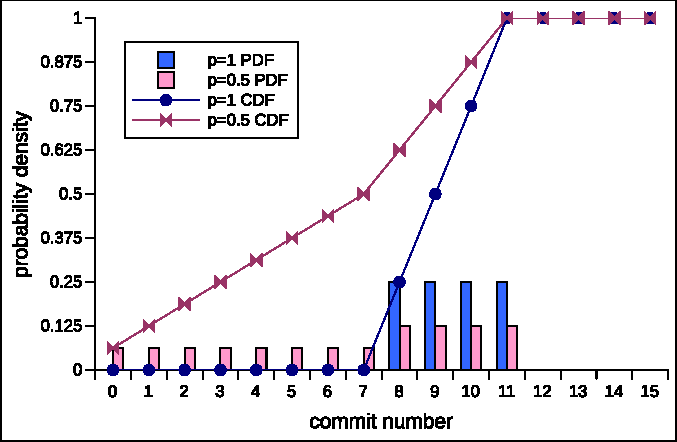
\includegraphics[width=0.45\textwidth]{example.pdf}
	\\
		(a) After two tests.
		\\
		\\

	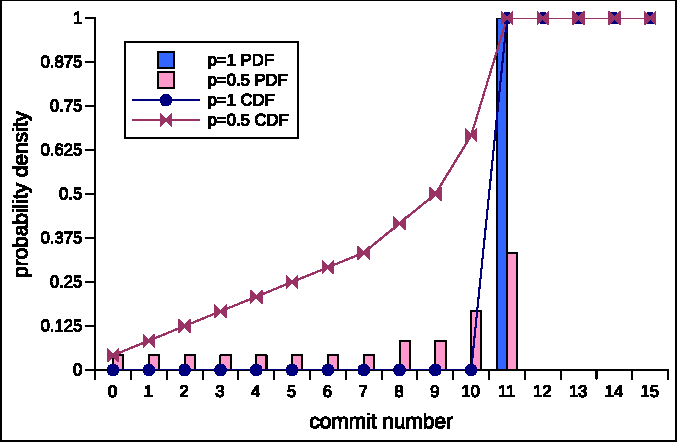
\includegraphics[width=0.45\textwidth]{example2.pdf}
	\\
		(b) After ``classical`` search terminates.
	\end{tabular}
	%\caption{Example deterministic and nondeterministic PDFs and CDFs.}
	\caption{Example \{,non\}deterministic \{P,C\}DFs.}
	\label{fig:example}
\end{figure}

A noteworthy invariant here is that the PDF is always monotonically nondecreasing in its nonzero range:
each passing test always shifts probability mass to the right of the bisect point,
but past the earliest known bug repro, nothing can ever revive it back above 0.

%%%%%%%%%%%%%%%%%%%%%%%%%%%%%%%%%%%%%%%%%%%%%%%%%%%%%%%%%%%%%%%%%%%%%%%%%%%%%%%%

\section{prior work}

I was kinda surprised to find no existing mathy solution to this problem lying around on the online.
Wikipedia has a brief little subsection on ``noisy binary search'', which links a few papers older than I am.
In one \cite{noisy2}, they bound the number of erroneous answers by a fixed factor of the number of queries,
so it's more like ``twenty questions with lies'' than bisect.
In another \cite{noisy1}, they do fix the error rate $p$,
but they allow for symmetric false negatives and false positives, both with the same $p$.
This too changes the nature of the problem;
notably, if $p=0.5$, you can't make any progress whatsoever.

Dropbox has a CI service called Athena \cite{athena}
which automatically searches for flaky tests, when otherwise no bug exists.
In this case the goal is to keep the build green, but if you consider the flaky test itself to be the bug, it's the same problem.%
\footnote{Incidentally, the symmetric case
-- where a bug repros with $p=1$, but the test also flakes with some $q<1$ --
is also the same problem.}
Athena's ``deflakes'' the test at each commit by running 10 times,
and treats the combined result as ``basically as good as $p=1$''.%
\footnote{Upcoming, I will call this strategy $\mathsf{Mistrustful(10)}$.}
In this setting, $p$ is not known in advance, so using Bayes's rule is off the table.
But I will show that even without access to the PDF, a better strategy exists. % at least by my definition

%%%%%%%%%%%%%%%%%%%%%%%%%%%%%%%%%%%%%%%%%%%%%%%%%%%%%%%%%%%%%%%%%%%%%%%%%%%%%%%%

\section{strategies}

Ok, so how do we
%cope with the fact that we'll never have a proper lower bound?
%How do we
make progress,
i.e., concentrate probability mass til there's $\confidents$ of it on one commit,
as quickly as possible?
%In principle, testing anywhere in the range $[0,b)$,
%where $b$ is the earliest known buggy commit,
%will make progress,
%
%% ghhh this sentence only feels good if i know what i'm talking about
%Let's deconstruct the motives of classical binary search.
Let $c_b$ be the earliest known buggy commit, and $c_a$ be the latest known safe commit.
In Determinism World, we would bisect at $c_{(a+b)/2}$
because that minimizes the maximum range remaining in the worst case outcome
(i.e., the two possible outcome ranges are the same length).
%But in Nondeterminism World,
%the worst case is a big constant times linear:
%an adversarial RNG god could pass your test a thousand times on $c_{n-1}$, then fail,
%then pass it a thousand times on $c_{n-2}$, then fail, and so on,
%before ultimately arriving at buggy commit $c_0$.
%So thinking about the worst case is not productive for a sublinear strategy,
%and also,
%we shouldn't be thinking about the range length,
%because a pass is still progress even though $a$ doesn't ever budge,
But in Nondeterminism World, $a$ doesn't ever budge from $0$,
so bisecting at $c_{(0+b)/2}$ will not even terminate.
%will eventually fail to make progress.
Sure, hitting the PDF with
%Bayes's rule at $b/2$
$\renorm{b/2}$
will always move {\it some} mass rightward,
but once five 9's of it is already over there,
%to the right of that point,
it can't concentrate it onto one point.
So let's not think about the range.

\subsection{bisect probability mass}

Another way to think about Determinism World is the $c_{(a+b)/2}$ bisect point
% maximizes the expected probability mass that moves from one side to the other.
cuts the probability mass, rather than the range, in half,
% How about in Nondeterminism World,
% we ignore the range length, and instead bisect at the midpoint of probability mass,
i.e., $\mathsf{last}_i \cdf(i) \le 0.5$.
This approach is compatible with Nondeterminism World,
fits the ``binary search'' spirit,
and will at least terminate
(if $b$ is the solution, it converges to repeatedly probing $b-1$),
which is more than you can say for the range-based $c_{(0+b)/2}$.
%It is intuitively obvious that this will make progress faster than bisecting at $c_{(b+0)/2}$,
%But is it fast?
However, it doesn't maximize either the minimum or the expected amount of mass that moves:
when $p<1$, it's intuitively easy to see that CDF threshold should actually be less than $0.5$.
\footnote{I did some pen-and-paper algebra to find a closed form for this,
but I actually trust the simulator more than myself at this point,
so I stopped spending brains on this part of the problem. I kind of regret that.}
% TODO TODO: actually do the paperwork.
Is maximizing the expected moved mass as a function of $p$ the fastest we can go,
and if so, why?

\subsection{bisect entropy}

\newcommand\entropy{\ensuremath{\mathcal{H}}\xspace}

A PDF's information content is measured in {\it entropy}:
$\entropy = \sum_i \pdf(i)\mathsf{ln}(\pdf(i))$.
Indeed,
in Determinism World the search terminates when $\entropy = 0$.
I thought for a while about how to link ``minimum expected entropy''
to the stated goal %in Nondeterminism World:
of
%minimizing the expected steps until
$\confidents = \mathsf{max}_i \pdf(i) \ge 0.99999$,
but couldn't really formalize the idea.
The goal of five 9's is fairly arbitrary anyway,
and also not necessarily stable under the entropy measurement,
since it doesn't care how the remaining $0.00001$ is distributed.
%
Also, a Very Smart Math Friend of mine was unable to find a simple closed form for
the expected resulting $\entropy(\renorm{} \circ \pdf)$
%\[
%(\cdf(j) + (1-\cdf(j))(1-p))\entropy(\renorm \circ \pdf)
%+
%p(1-\cdf(j))\entropy(\renorm{\text{bug}} \circ \pdf)
%\]
or whatever (bleh, my notation is kinda reaching its limits here).
%so how would you write a proof about it anyway.
Nevertheless, it seems promising, and easy to implement.

\subsection{bisect randomly}

Maybe a random world calls for a random algorithm!
It's obvious this will terminate, but of course it won't be fast.
Intuitively, if we use the PDF to weight the random choice, it will be faster than choosing uniformly in $[0,b)$.
But how much faster?

You can tell it's at this point I'm starting to get statistics fatigue.

\subsection{human}

Humans are known to be less patient than computers (citation: see previous sentence).
If a human is unwilling to compute $\renorm{} \circ \pdf$ by hand every step,
or, more prohibitively,
simply doesn't know $p$ in advance so can't compute $\renorm{}$ at all,
what should they do?

Think back to Athena from the prior work section.
The human

Regardless, it's easy to 


%(
% hmmm...


% In Determinism World, the search terminates when 

% Let's think of bisecting at $c_{(a+b)/2}$, in Determinism World, 
% as maximizing the expected information gained from either test result.
% On PDFs, information gain is measured as 





%%%%%%%%%%%%%%%%%%%%%%%%%%%%%%%%%%%%%%%%%%%%%%%%%%%%%%%%%%%%%%%%%%%%%%%%%%%%%%%%

\section{simulating it}

At this point I threw in the towel on the maths front,
and wrote a bunch of code to let the law of large numbers do my work for me.

\cite{drowningpoint}
\cite{epsilon}

%%%%%%%%%%%%%%%%%%%%%%%%%%%%%%%%%%%%%%%%%%%%%%%%%%%%%%%%%%%%%%%%%%%%%%%%%%%%%%%%

\section{evaluation}

%%%%%%%%%%%%%%%%%%%%%%%%%%%%%%%%%%%%%%%%%%%%%%%%%%%%%%%%%%%%%%%%%%%%%%%%%%%%%%%%

\section{future work}

% weigh cost of running test suite vs cost of git checkout -- mistrustful() gets a whole lot better! but, where is the break even point when you should git checkout?

% p not known, figur eit out on the fly

%%%%%%%%%%%%%%%%%%%%%%%%%%%%%%%%%%%%%%%%%%%%%%%%%%%%%%%%%%%%%%%%%%%%%%%%%%%%%%%%

\section{conclusion}



\acks

Thanks to Jason Reed, Lynn Chordbug, and Sujay Jayakar for thinking about this problem with me.

%%%%%%%%%%%%%%%%%%%%%%%%%%%%%%%%%%%%%%%%%%%%%%%%%%%%%%%%%%%%%%%%%%%%%%%%%%%%%%%%

\renewcommand{\refname}{references}
\bibliographystyle{abbrvnat}
\bibliography{citations}

\end{document}
